%!TEX root = ../report.tex

\begin{document}
    \chapter{Results and Evaluation}

    In this chapter, the results of the registration of the available data using the solution presented in \autoref{chap:Solution} will be presented and discussed.
    The data was visulized with the 3D visualization provided by Open3D. 

%-------------------------------------------------------------------------------
%	Registration of a CityGML model with a point cloud
%-------------------------------------------------------------------------------
    \section{Registration of a CityGML model with a point cloud}
        The initial pose of the CityGML model and the point cloud can be found in \autoref{fig:initial_front_model} and \autoref{fig:initial_back_model}.
        \autoref{fig:initial_front_model} shows a front view of the fire exercise building in Dortmund, while \autoref{fig:initial_back_model} shows a back view.

        The result after the registration is showed in \autoref{fig:final_front_model} and \autoref{fig:final_back_model}.
        After the resultin

        \begin{figure}[H]
            \centering
            \begin{subfigure}{1\textwidth}
                \centering
                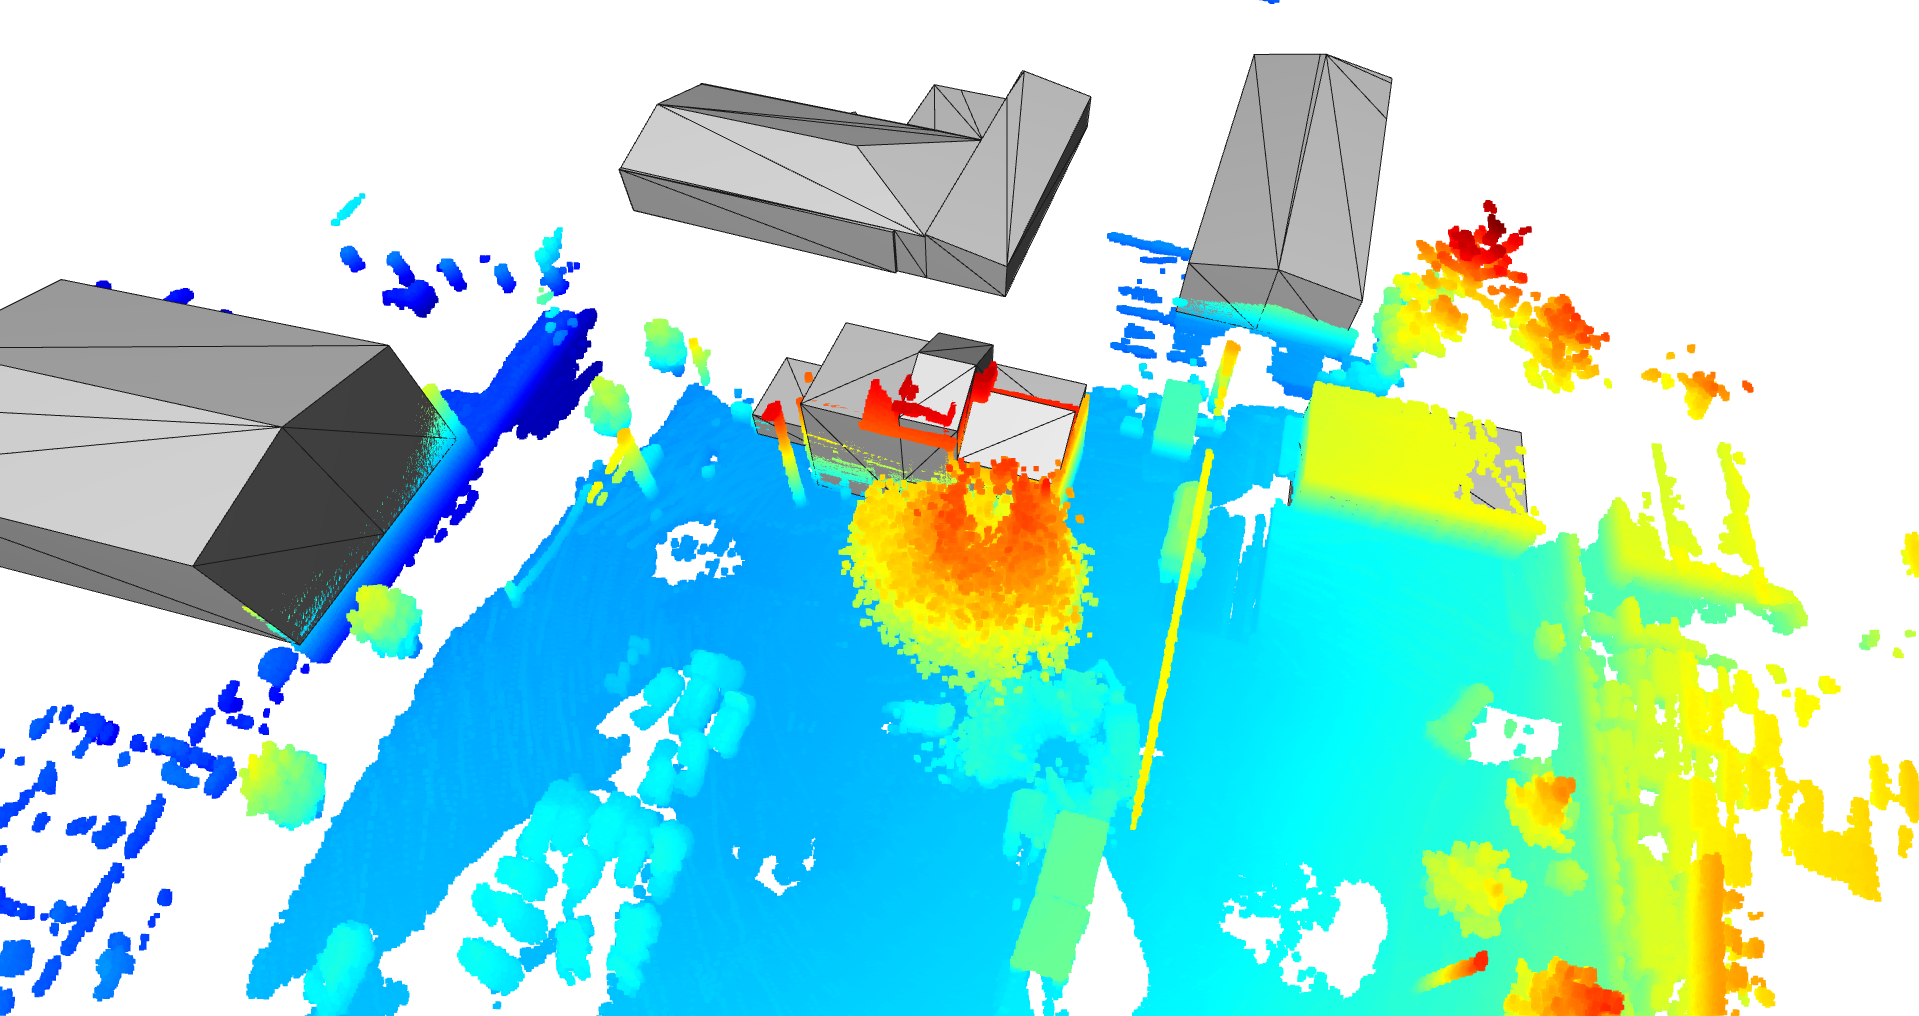
\includegraphics[scale=0.2]{images/solution_images/final_front.png}
                \caption{Front view of a point cloud and a CityGML model after registration.}
                \label{fig:final_front_model}
            \end{subfigure}
            \hfill
            \begin{subfigure}{1\textwidth}
                \centering
                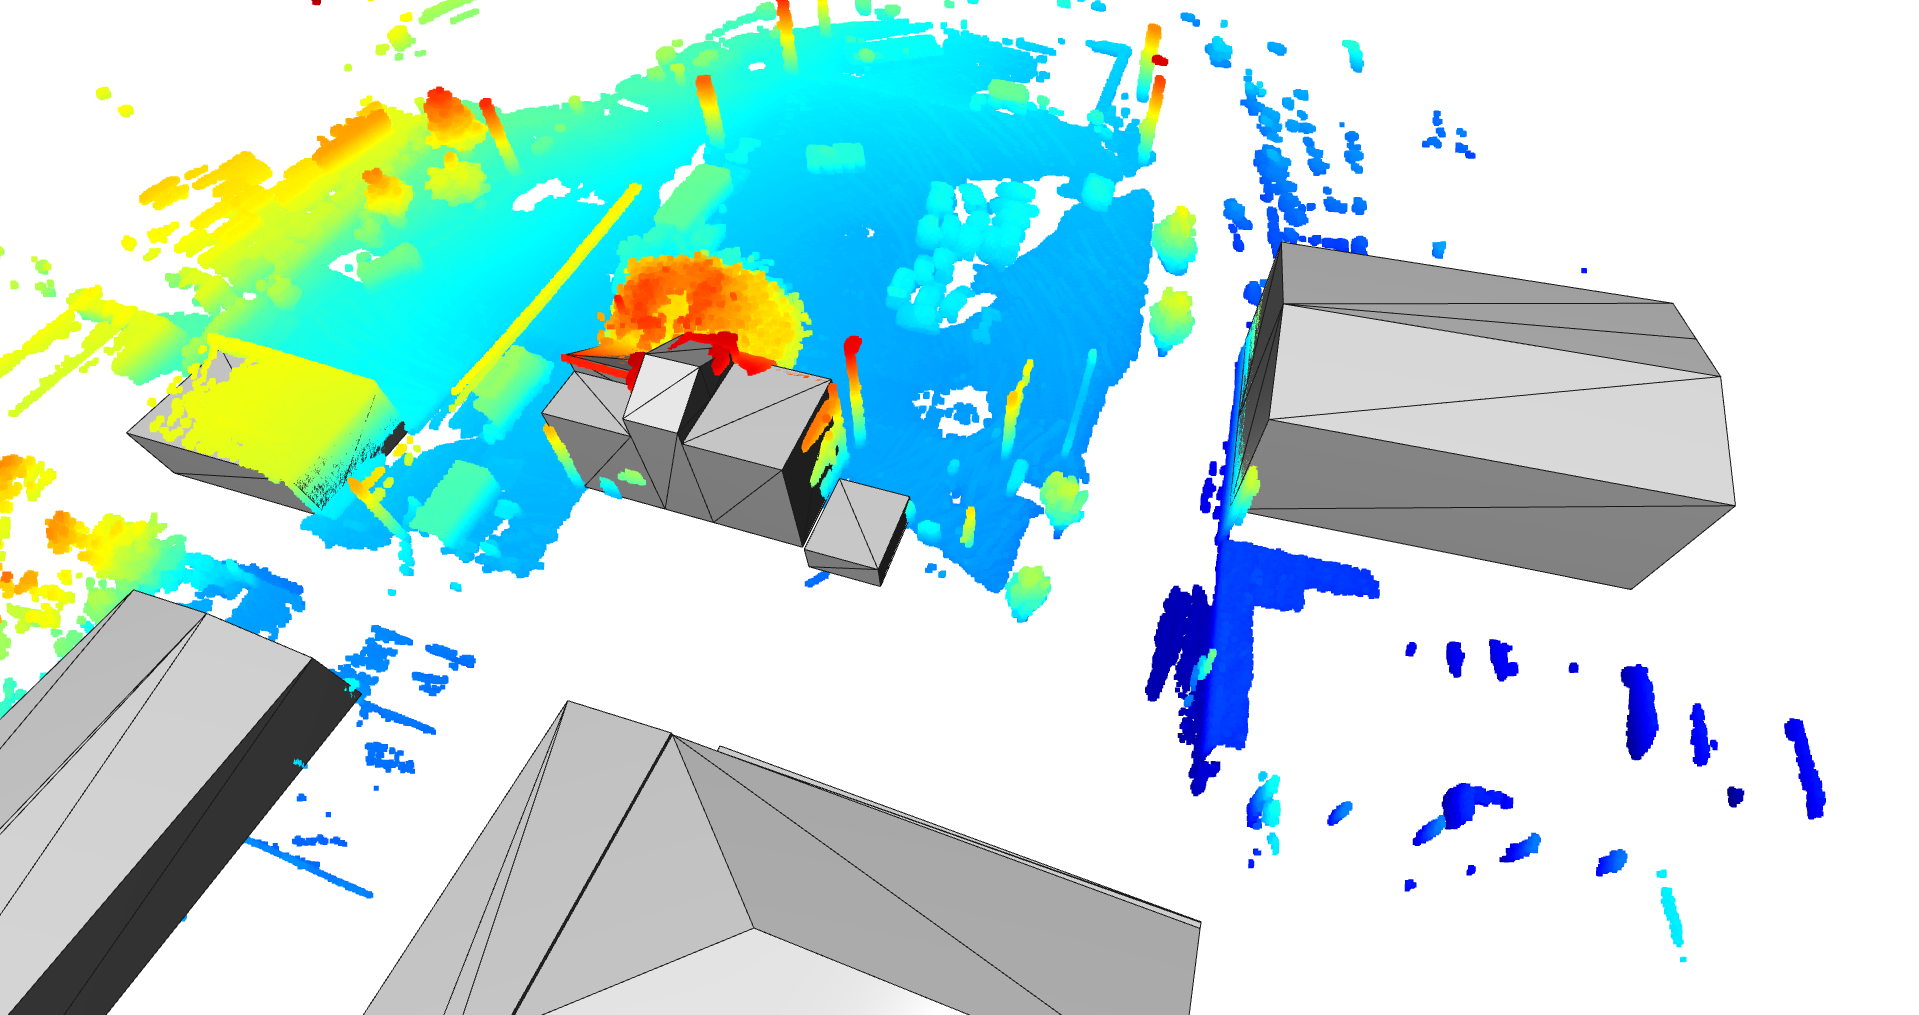
\includegraphics[scale=0.2]{images/solution_images/final_back.png}
                \caption{Back view of a point cloud and a CityGML model after registration.}
                \label{fig:final_back_model}
            \end{subfigure}
            \caption{A figure with two subfigures}
            \label{fig:final_CityGML}
        \end{figure}

%-------------------------------------------------------------------------------
%	Registration of a PLY model with a point cloud
%-------------------------------------------------------------------------------
    \section{Registration of a PLY model with a point cloud}
        \begin{figure}[H]
            \centering
            \begin{subfigure}{1\textwidth}
                \centering
                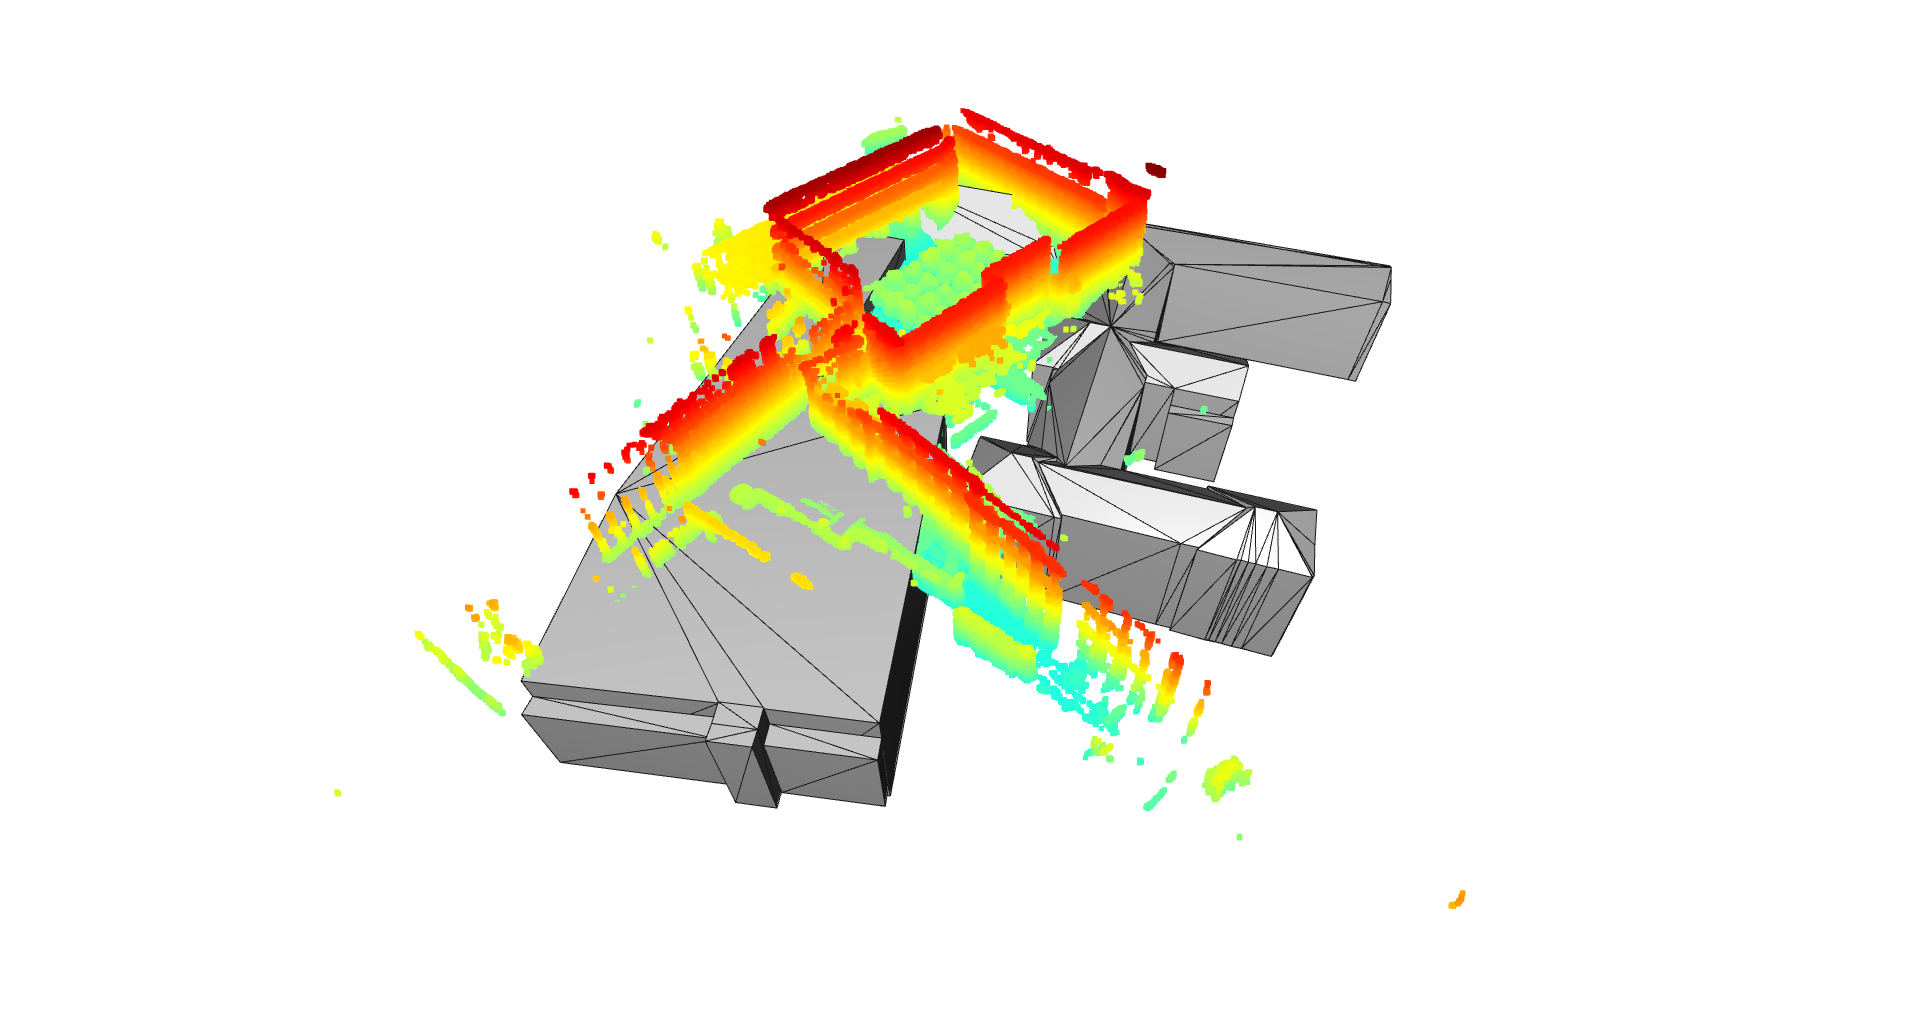
\includegraphics[scale=0.2]{images/solution_images/initial_ply_a.png}
                \caption{Front view a point cloud and a PLY model before registration.}
                \label{fig:intial_ply_a}
            \end{subfigure}
            \hfill
            \begin{subfigure}{1\textwidth}
                \centering
                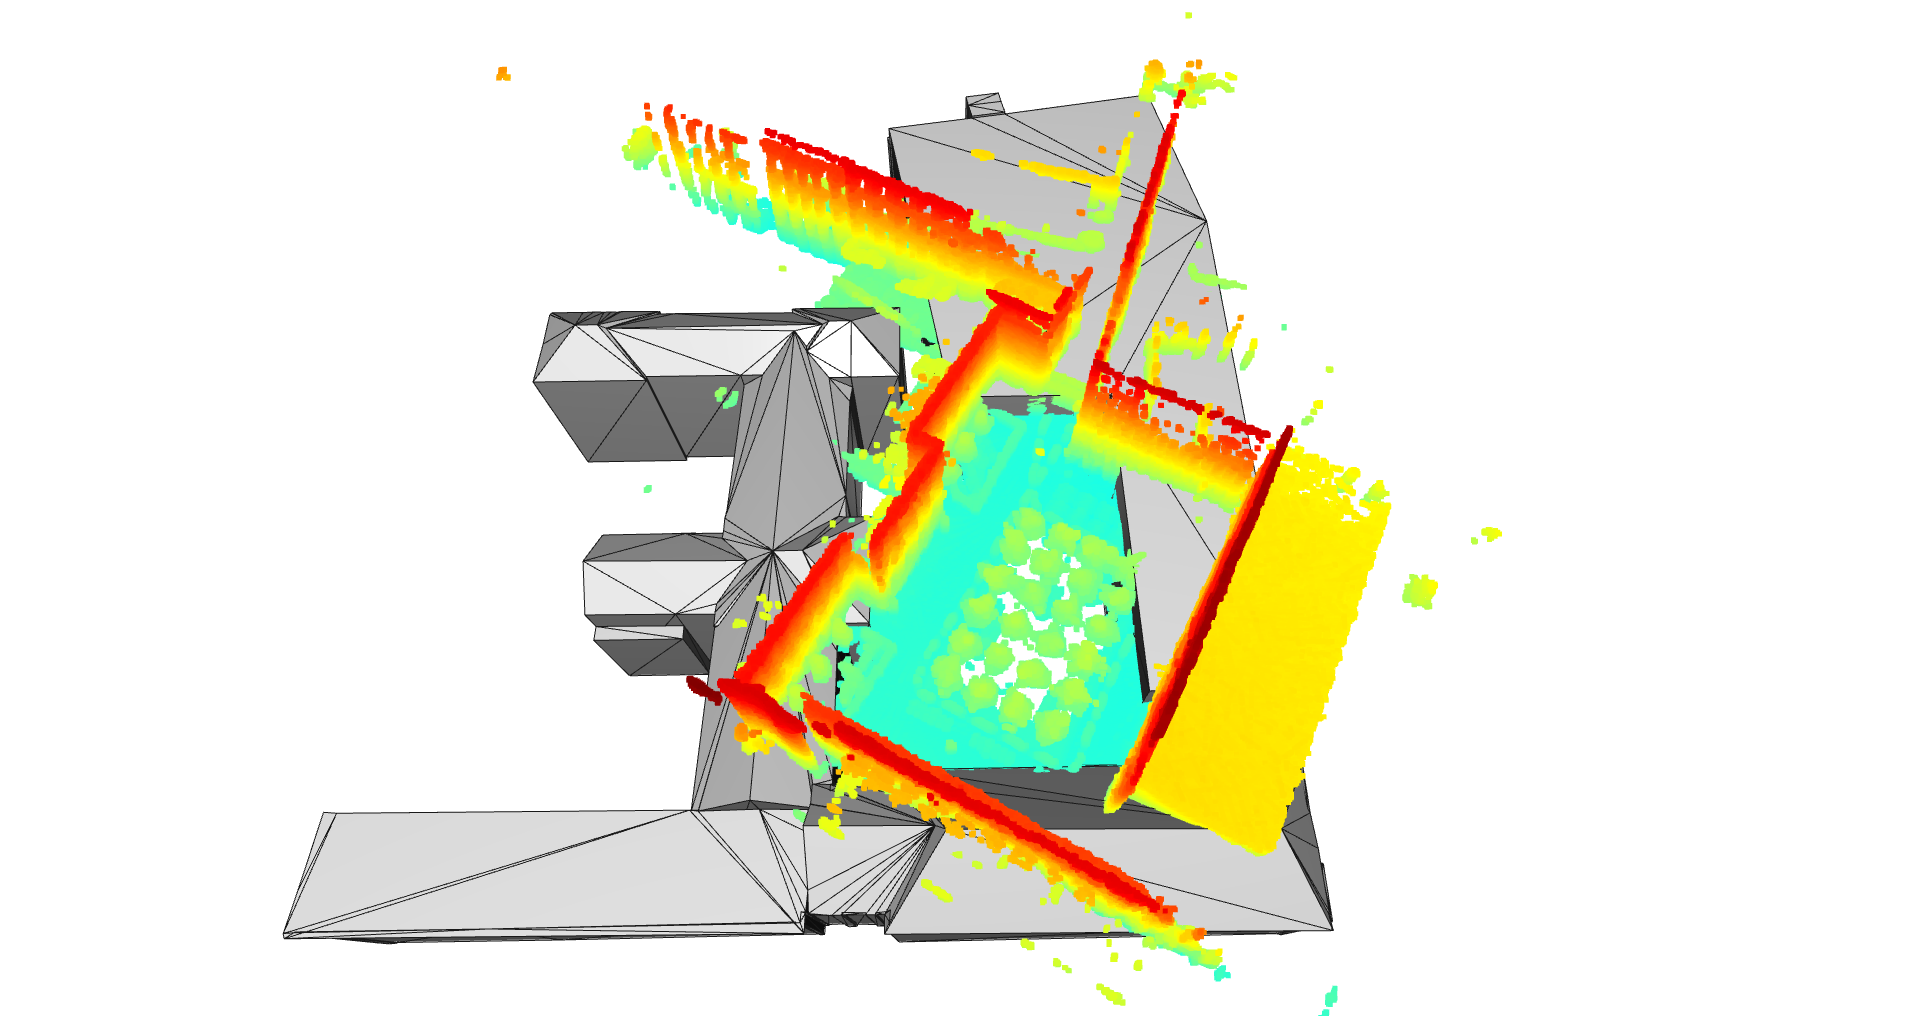
\includegraphics[scale=0.2]{images/solution_images/initial_ply_b.png}
                \caption{Back view of a point cloud and a PLY model before registration.}
                \label{fig:intial_ply_b}
            \end{subfigure}
            \caption{A figure with two subfigures}
            \label{fig:initial_ply}
        \end{figure}

        
        \begin{figure}[H]
            \centering
            \begin{subfigure}{1\textwidth}
                \centering
                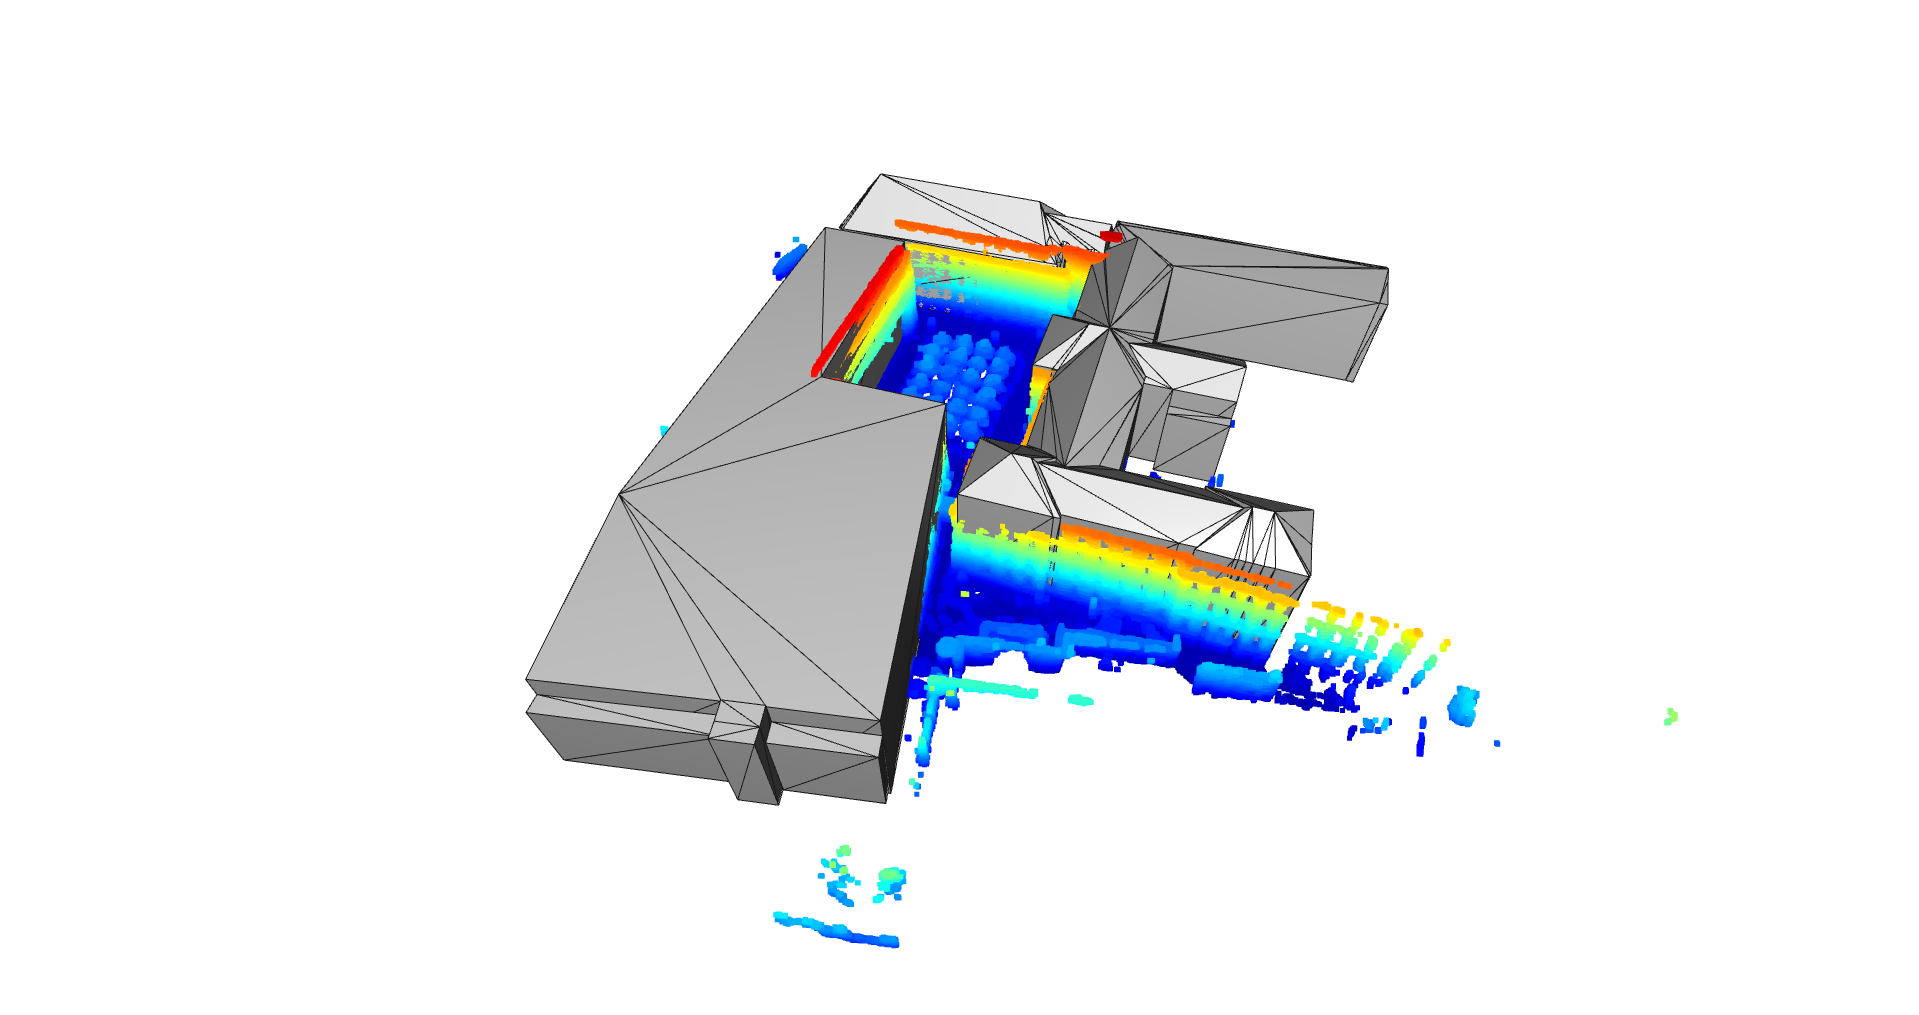
\includegraphics[scale=0.2]{images/solution_images/final_ply_a.png}
                \caption{Front view a point cloud and a PLY model after registration.}
                \label{fig:final_ply_a}
            \end{subfigure}
            \hfill
            \begin{subfigure}{1\textwidth}
                \centering
                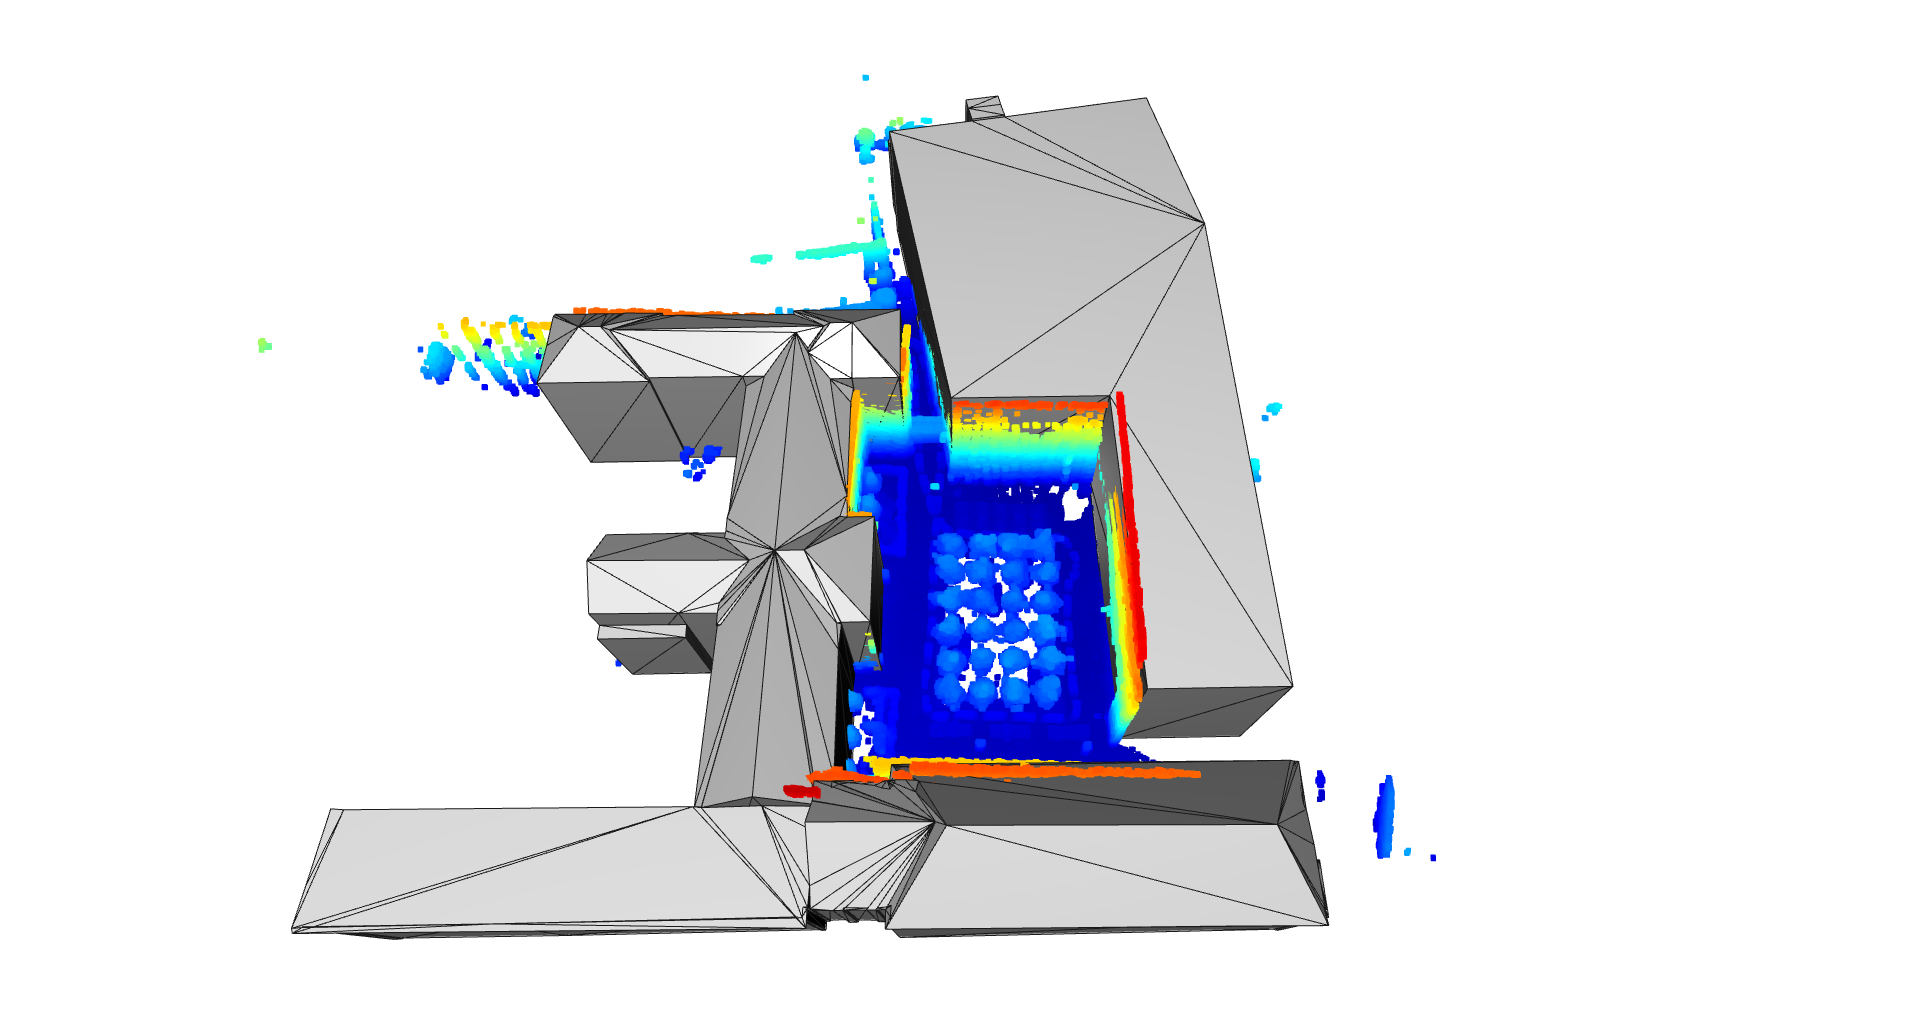
\includegraphics[scale=0.2]{images/solution_images/final_ply_b.png}
                \caption{Back view of a point cloud and a PLY model after registration.}
                \label{fig:final_ply_b}
            \end{subfigure}
            \caption{A figure with two subfigures}
            \label{fig:final_ply}
        \end{figure}


    
\end{document}
